\section{Model Inversion Attacke}\label{sec:model_inversion}

Bei der Model Inversion Attacke, versucht ein Angreifer, durch bestimmte Eingaben in das Modell, Rückschlüsse zu den Trainingsdaten zu ziehen. Dies kann soweit führen, dass einzelne Datenpunkte nachgebildet werden können \cite{P-3}. 

Fredrikson et al. \cite{P-3} zeigen anhand eines Gesichterkennungsmodells, dass es möglich ist, das Bild einer Person zu rekonstruieren.
Diese Person muss lediglich von dem Modell klassifiziert werden können, folglich also auch in den Trainingsdaten vorhanden sein.
Abbildung \ref{fig:mi_attacke} zeigt, wie sehr das rekonstruierte Bild (links) dem Originalbild (rechts) ähnelt.

\begin{figure}[!htb]
    \centering
    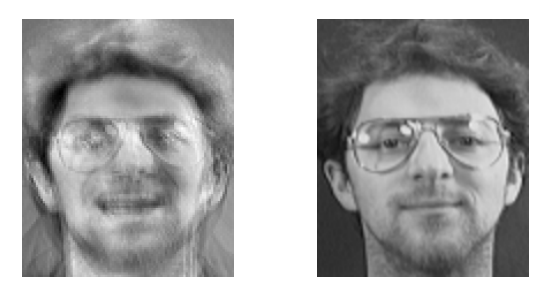
\includegraphics[width=8cm]{figures/mi_attack}
    \caption{Rekonstruktion eines Bildes \cite{P-3}}
    \label{fig:mi_attacke}
\end{figure} 

Der Angriff, auch Reconstruction Attacke genannt, wird durch einen generativen, iterativen Algorithmus durchgeführt.
Zu Beginn wird ein Bild als Startbild gesetzt, welches jedem Pixel den Wert 0 zuweist.
In jedem Schritt des Algorithmus wird zuerst der Wert einer Verlustfunktion bestimmt.
Der Wert dieser ist, sofern das Modell nicht mehr Details angibt, lediglich der Confidence Score, dass es sich bei dem eingegebenen Bild nicht um das gesuchte Label handelt.
Konkret bedeutet dies, wenn das Bild bereits die zu rekonstruierende Person zeigt, der Confidence Score des Labels der Person nahe 1 ist und damit unsere Verlustfunktion nahe 0.
Anschließend wird das Bild des vorherigen Durchlaufs, durch einen Autoencoder geschickt, welcher ein Bild für den nächsten Schritt des Algorithmus erzeugt.
Bei diesem Autoencoder handelt es sich um ein Neuronales Netz, welches einen Input (hier ein Bild) in einen Vektor mit niedrigerem Rang transformiert und anschließend wieder in einen Vektor mit dem gleichen Rang wie den Input transformiert.
Input und Output eines Autoencoders haben somit den gleichen Rang, hier wird also ein Bild zu einem anderen Bild transformiert.
Zum Training des Autoencoders werden Bilder genutzt, wobei der Input auch gleich dem Output entspricht. 
Somit lernt ein Autoencoder, aus einem Bild das gleiche Bild zu erzeugen, jedoch mit der Einschränkung, dass der Vektor innerhalb des Modells einen niedrigen Rang hat.
Dieser Algorithmus läuft so lange, bis die maximal konfigurierte Anzahl an Schritten erreicht wurde, die Verlustfunktion einen bestimmten Wert überschritten hat oder sich eine definierte Anzahl an Schritten lang nichts verbessert hat.

Zhang et al. \cite{P-4} erweitern diesen Angriff, indem die Qualität des generativen Modells (Autoencoder) verbessert wird. 
Zum einen wird der Autoencoder so erweitert, dass zusätzliche Informationen mitgegeben werden können. 
Diese zusätzlichen Informationen sind beispielsweise verschwommene oder zensierte Bilder. 
Eine weitere Verbesserung besteht darin, zusätzlich ein Modell zu nutzen, welches reale Bilder von synthetischen Bildern unterscheiden soll.
Dieses Konstrukt entspricht dem Diskriminator eines Generative Adversarial Networks \cite{P-86}.
Mithilfe des Diskriminators, kann der Autoencoder verbessert werden, wodurch die Qualität der einzelnen Bilder erhöht wird und folglich auch die Qualität des rekonstruierten Bildes steigt.

He et al. \cite{P-5} zeigen eine White Box Version des Angriffs. 
White Box bedeutet, dass das Modell vollumfänglich in den Händen des Angreifers ist.
Dies ist der Fall, wenn ein Modell öffentlich geteilt wird (die Trainingsdaten jedoch nicht).
Die Fähigkeit, das Modell vollumfänglich zu nutzen, erlaubt es, das zu rekonstruierende Bild mittels Backpropagation anzupassen. 
Dazu wird initial ein Bild genutzt, bei jedem jeder Pixel auf einen einheitlichen Farbwert, z. B. 0.5, gesetzt wird.
Dieses Bild wird nun durch das Modell interferiert, und der Wert der Verlustfunktion wird backpropagiert. 
Alle Gewichte und Bias des Modells werden dabei unverändert gelassen, jedoch werden die Pixel des Bildes Gradienten bestimmt und mit einer konfigurierten Lernrate angepasst.
Dieser Vorgang wird anschließend so lange wiederholt, bis eine maximale Anzahl an Iterationen durchgelaufen ist.

